\documentclass[
ngerman,
twoside,
pdfa=false,
ruledheaders=section,%Ebene bis zu der die Überschriften mit Linien abgetrennt werden, vgl. DEMO-TUDaPub
class=report,% Basisdokumentenklasse. Wählt die Korrespondierende KOMA-Script Klasse
thesis={type=sta},% Dokumententyp Thesis, für Dissertationen siehe die Demo-Datei DEMO-TUDaPhd
accentcolor=TUDa-2c,% Auswahl der Akzentfarbe
custommargins=false,% Ränder werden mithilfe von typearea automatisch berechnet
marginpar=false,% Kopfzeile und Fußzeile erstrecken sich nicht über die Randnotizspalte
%BCOR=5mm,%Bindekorrektur, falls notwendig
parskip=half-,%Absatzkennzeichnung durch Abstand vgl. KOMA-Sript
fontsize=11pt,%Basisschriftgröße laut Corporate Design ist mit 9pt häufig zu klein
%	logofile=tuda_logo.pdf, %Falls die Logo Dateien nicht installiert sind
]{tudapub}

%%%%%%%%%%%%%%%%%%%%%%%%%%%%
% Download des TU-Logos
%%%%%%%%%%%%%%%%%%%%%%%%%%%%
% https://download.hrz.tu-darmstadt.de/protected/CE/TUDa_LaTeX/tuda_logo.pdf
% Der Pfad zum Logo kann als "logofile" angegeben werden.

%%%%%%%%%%%%%%%%%%%
% Sprachanpassung & Verbesserte Trennregeln
%%%%%%%%%%%%%%%%%%%
\usepackage[english, main=ngerman]{babel}
\usepackage[autostyle]{csquotes}% Anführungszeichen vereinfacht
\usepackage{microtype}

%%%%%%%%%%%%%%%%%%%
% Literaturverzeichnis
%%%%%%%%%%%%%%%%%%%
\usepackage{biblatex}   % Literaturverzeichnis
\addbibresource{HausarbeitBib.bib}

%%%%%%%%%%%%%%%%%%%
% Paketvorschläge Tabellen
%%%%%%%%%%%%%%%%%%%
%\usepackage{array}     % Basispaket für Tabellenkonfiguration, wird von den folgenden automatisch geladen
\usepackage{tabularx}   % Tabellen, die sich automatisch der Breite anpassen
%\usepackage{longtable} % Mehrseitige Tabellen
%\usepackage{xltabular} % Mehrseitige Tabellen mit anpassarer Breite
\usepackage{booktabs}   % Verbesserte Möglichkeiten für Tabellenlayout über horizontale Linien

%%%%%%%%%%%%%%%%%%%
% Paketvorschläge Mathematik
%%%%%%%%%%%%%%%%%%%
\usepackage{mathtools} % erweiterte Fassung von amsmath
\usepackage{amssymb}   % erweiterter Zeichensatz
\usepackage[decimalsymbol=comma]{siunitx}   % Einheiten


%%%%%%%%%%%%%%%%%
% Eigenen Pakete Gruppe03
%%%%%%%%%%%%%%%%%%%%
%\usepackage[utf8]{inputenc}
%\usepackage[ngerman]{babel}
\usepackage{hyperref}
\usepackage{graphicx}
\usepackage{subcaption}
\usepackage{listings}
\usepackage[framed, numbered]{matlab-prettifier}
%\usepackage[style=numeric]{biblatex}
%\usepackage{amsthm}
%\usepackage[squaren]{SIunits}
\usepackage{enumitem}
\usepackage{tikz}
\usepackage{pgfplots}
\usepackage{pgfplotstable}
%\usepackage{booktabs}
\pgfplotsset{compat=1.12}
\usepackage{dsfont}

%%%%%%%%%%%%%%%%%%%
% Pseudocode
%%%%%%%%%%%%%%%%%%%
\usepackage[linesnumbered,lined,boxruled]{algorithm2e} % Package für Pseudocode

%%%%%%%%%%%%%%%%%%%
% Plotting und Grafik
%%%%%%%%%%%%%%%%%%%
\usepackage{tuda-pgfplots} % Package für Plotting with TUDa mods

%%%%%%%%%%%%%%%%%%%
% Sonstiges
%%%%%%%%%%%%%%%%%%%
\usepackage{blindtext} % Package für Blindtext


%%%%%%%%%%%%%%%%%%%
%setzt floats auch oben auf die seite
%%%%%%%%%%%%%%%%%%%
\makeatletter
\setlength{\@fptop}{0pt}
\setlength{\@fpbot}{0pt plus 1fil}
\makeatother


\begin{document}
	\title{Ausarbeitung Übung 5}
	%\subtitle{Ein Untertitel, wenn nötig}
	\author[D. Schiller, C. Kramer, S.Arnold, T. Lingenberg]{Dominik Schiller \and Constanze Kramer \and Simon Arnold \and Tobias Lingenberg} %optionales Argument ist die Signatur,
	%\reviewer{Gutachter 1 \and Gutachterin 2} %Gutachten
	
	%Diese Felder werden untereinander auf der Titelseite platziert.
	\department{} % Das Kürzel wird automatisch ersetzt und als Studienfach gewählt, siehe Liste der Kürzel im Dokument.

	
	\date{\today}
	%\examdate{\today}
	
	%	\tuprints{urn=1234,printid=12345}
	%	\dedication{Für alle, die \TeX{} nutzen.}
	
	\maketitle
	\pagenumbering{gobble} % Seitenzahlen angezeigt, startet ab dem Inhaltsverzeichnis
	
	
	%\affidavit
	%\AffidavitSignature
	%\AffidavitSignature
	
	
	%%%%%%%%%%%%%%%%%%%
	%Abstract / Kurzzusammenfassung
	%%%%%%%%%%%%%%%%%%%
	%\include{chapters/zusammenfassung}
	
	%%%%%%%%%%%%%%%%%%%
	%Inhaltsverzeichnis 
	%%%%%%%%%%%%%%%%%%%
	\cleardoublepage
	\tableofcontents % Erstellte ein Inhaltsverzeichnis
	
	%\cleardoublepage
	\pagenumbering{arabic} % Seitenzahlen angezeigt, startet ab dem Inhaltsverzeichnis
	\setcounter{page}{1} % Setzt den Seitenzahlenzähler auf 1
	
	%%%%%%%%%%%%%%%%%%%%%%%%%%%%%%%%%%%%%%%%%%%%%%%%%%%%%%%%%%%%%%%%%%%%%%%%%%%%%%%%%%%%%%%%%%%%%%%%%%
	
	% INHALT, am Besten ausgelagert in eigene Files/Kapitel und dann mit \include{Unterordner/Filename} eingefügt, sorgt für bessere Übersichtlichkeit und Fehlersuche. Einzelne Dateien sind aktuell im Ordner Sections abgelegt. 
	
	
	%%%%%%%%%%%%%%%%%%Haupteil%%%%%%%%%%%%%%%%%%%
	\chapter{Bearbeitung der Aufgaben}
\section{Geschichteter Plattenkondensator}

Um numerisch die Kapazität eines Plattenkondensators mit quer geschichteten Dielektrika, die eine linear steigende relative Permittivität aufweisen, zu bestimmen, kann man den linearen Verlauf über mehrere Schichten mit jeweils konstanter Permittivität approximieren. Wie bei numerischen Verfahren üblich wird die Approximation besser, je dünner die einzelnen Schichten gewählt werden.\\
\begin{figure}[h!]
	\centering
	\begin{subfigure}[h]{0.3\textwidth}
		\centering
		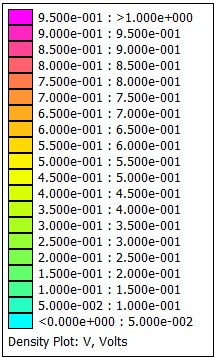
\includegraphics[width=\textwidth]{data/KondensatorN9_Legende}
		\caption{Skala}
		\label{fig:Skala1}
	\end{subfigure}
	\begin{subfigure}[h]{0.51\textwidth}
		\centering
		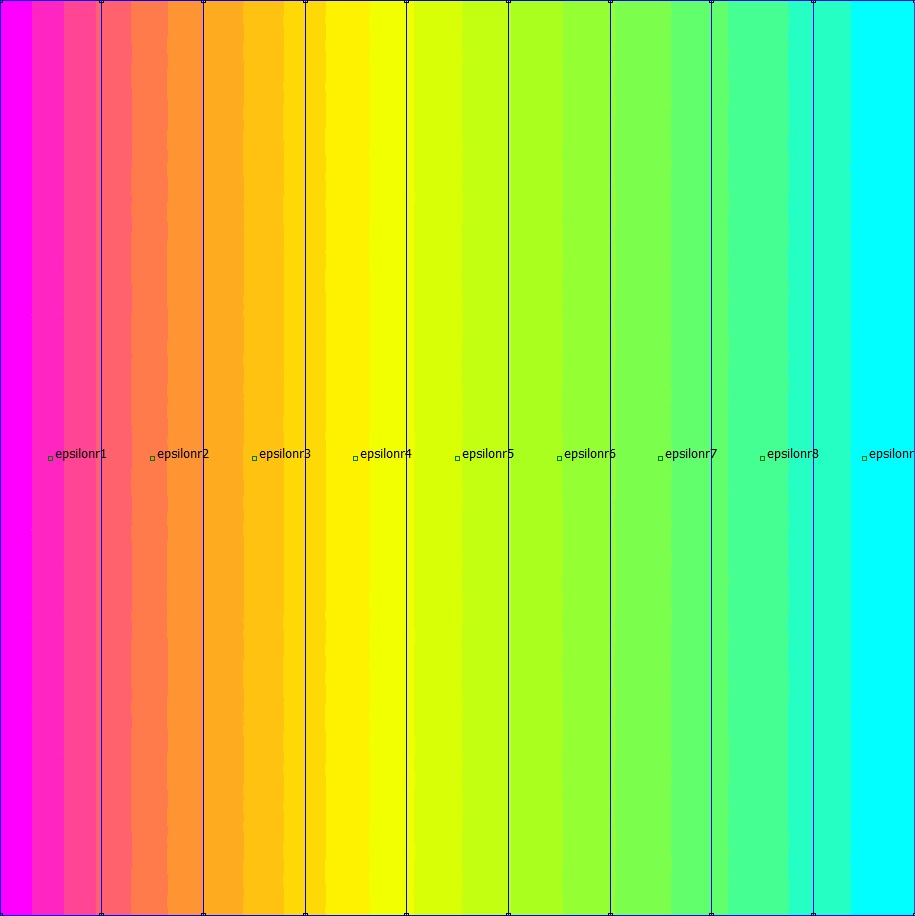
\includegraphics[width=\textwidth]{data/KondensatorN9}
		\caption{Potentialverlauf im Plattenkondensator mit 9 Schichten}
		\label{fig:N9}
	\end{subfigure}
	\caption{Potentialverlauf im Plattenkondensator mit 9 Schichten}
\end{figure} \\
Die Funktion \texttt{femmcapacity.m} bekommt als Parameter den Abstand $h$ zwischen den beiden Platten des Kondensators, die Kantenlänge $a$ der quadratischen Platten, $\varepsilon_{\mathrm{r,1}}$, $\varepsilon_{\mathrm{r,2}}$ und die Anzahl $N$ an Schichten übergeben. Mit Hilfe dieser Parameter wird daraus ein Plot für den Potentialverlauf im Kondensator erzeugt und die Kapazität der Anordnung berechnet. Die relative Permittivität variiert hierbei linear zwischen $\varepsilon_{\mathrm{r,1}} $ am linken Rand und $\varepsilon_{\mathrm{r,2}}$ am rechten Rand. Die zugehörigen Werte der relativen Permittivitäten der einzelnen Schichten $N_i$ lassen sich mit $$ \varepsilon_{\mathrm{r,i}} = \varepsilon_{\mathrm{r,1}} + \frac{i (\varepsilon_{\mathrm{r,2}}-\varepsilon_{\mathrm{r,1}})}{N-1}$$ berechnen. Im Folgenden wird der Abstand zwischen den Platten und die Kantenlänge mit \SI{30}{\centi\meter} angenommen. Wählt man 9 Schichten, $\varepsilon_{\mathrm{r,1}} = 1$ und $\varepsilon_{\mathrm{r,2}} = 2$  erhält man den in Abbildung \ref{fig:N9} zu sehenden Potentialverlauf und eine Kapazität $ C_1 = \SI{3,793}{\pico\farad}$.\\ \\
Wiederholt man die Simulation für $N = 1,2,3,...,20$ Schichten und lässt sich in einem Konvergenz-Plot (Abbildung \ref{fig:semilogy}) die Kapazität in Abhängigkeit der Schichtanzahl anzeigen, wird deutlich, dass schon nach $N=3$ Schichten die Kapazität annähernd exakt bestimmt wird und weitere Verfeinerungen nur noch marginale Verbesserungen der Approximation erzielen. \\ \\

\begin{figure}[tpbh]
	\centering
	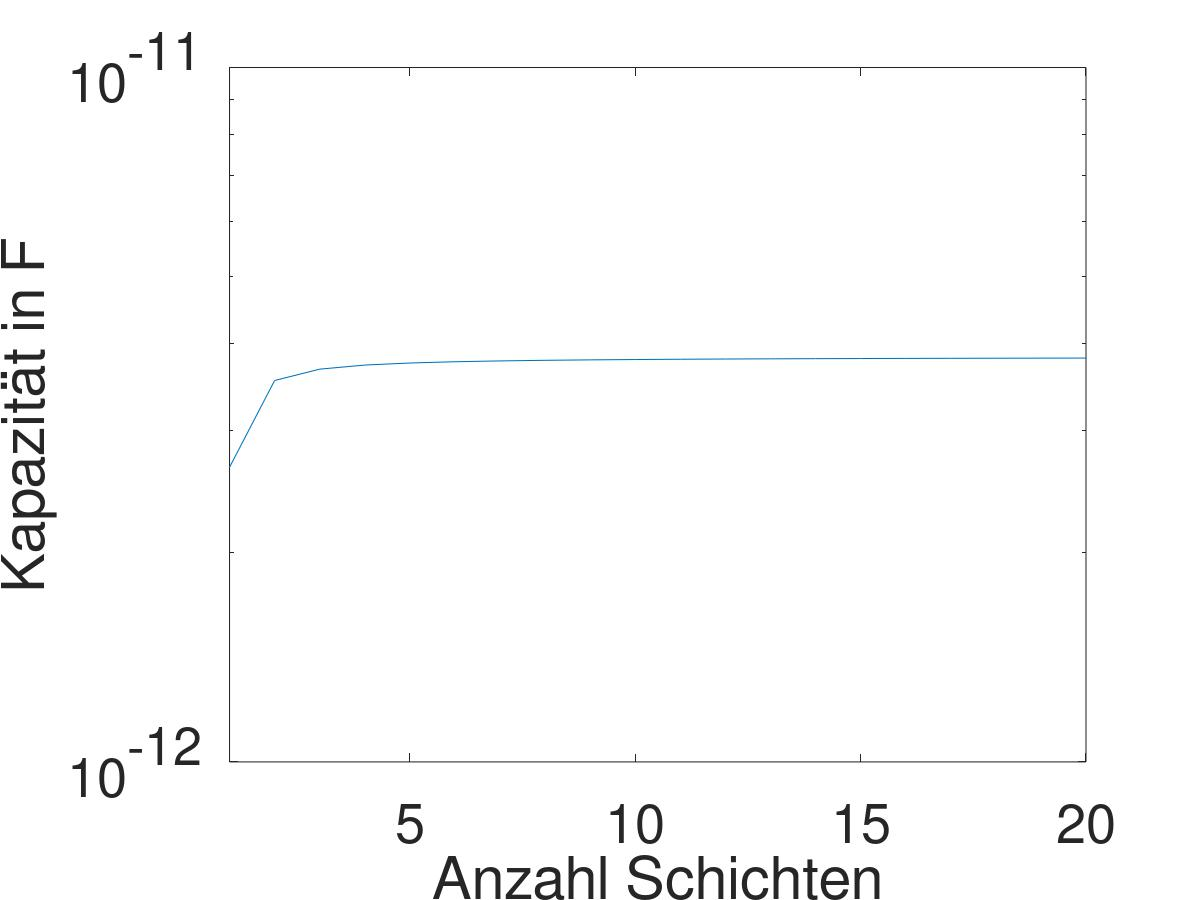
\includegraphics[width=.8\textwidth]{data/Kapazitaet}
	\caption{Änderung der Kapazität mit steigender Anzahl an Schichten im Plattenkondensator}
	\label{fig:semilogy}
\end{figure}


Die Option \texttt{'Vector Plot'} in FEMM ist nützlich, um den Verlauf des elektrischen Feldes besser darzustellen. Die Richtung der Pfeile zeigt an in welche Richtung das Feld an dieser Stelle zeigt und die Länge der Pfeile deutet die Stärke an dieser Stelle an.
\newpage
In Abbildung \ref{fig:N1_EFeld} sieht man den Plot für den homogenen Plattenkondensator und in Abbildung \ref{fig:N9_EFeld} für den geschichteten Fall. Vergleicht man beide Abbildungen fällt auf, dass das elektrische Feld im homogenen Plattenkondensator homogen verteilt ist. Beim geschichteten Plattenkondensator hingegen ist das elektrische Feld deutlich stärker auf der Seite mit der geringeren relativen Permittivität und nimmt immer weiter ab, je höher die relative Permittivität ist.

\begin{figure}[h]
	\begin{subfigure}[c]{0.2\textwidth}
		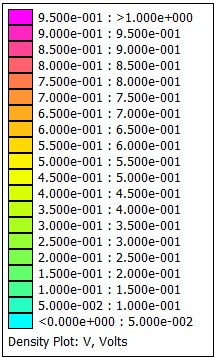
\includegraphics[width=\textwidth]{data/KondensatorN9_Legende}
		\caption{Skala}
		\label{fig:Skala2}
	\end{subfigure}
	\begin{subfigure}[c]{0.35\textwidth}
		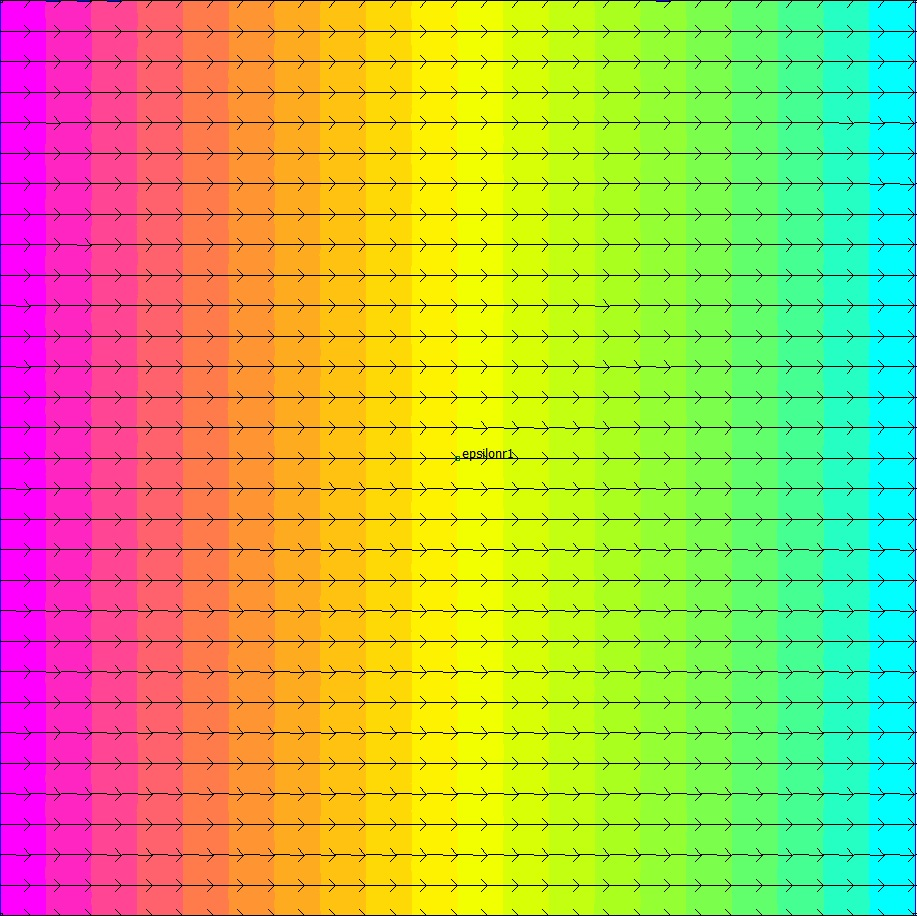
\includegraphics[width=\textwidth]{data/KondensatorN1_EFeld}
		\caption{Potentialverlauf und elektrische Feldstärke im homogenen Plattenkondensator}
		\label{fig:N1_EFeld}
	\end{subfigure}
	\begin{subfigure}[c]{0.35\textwidth}
		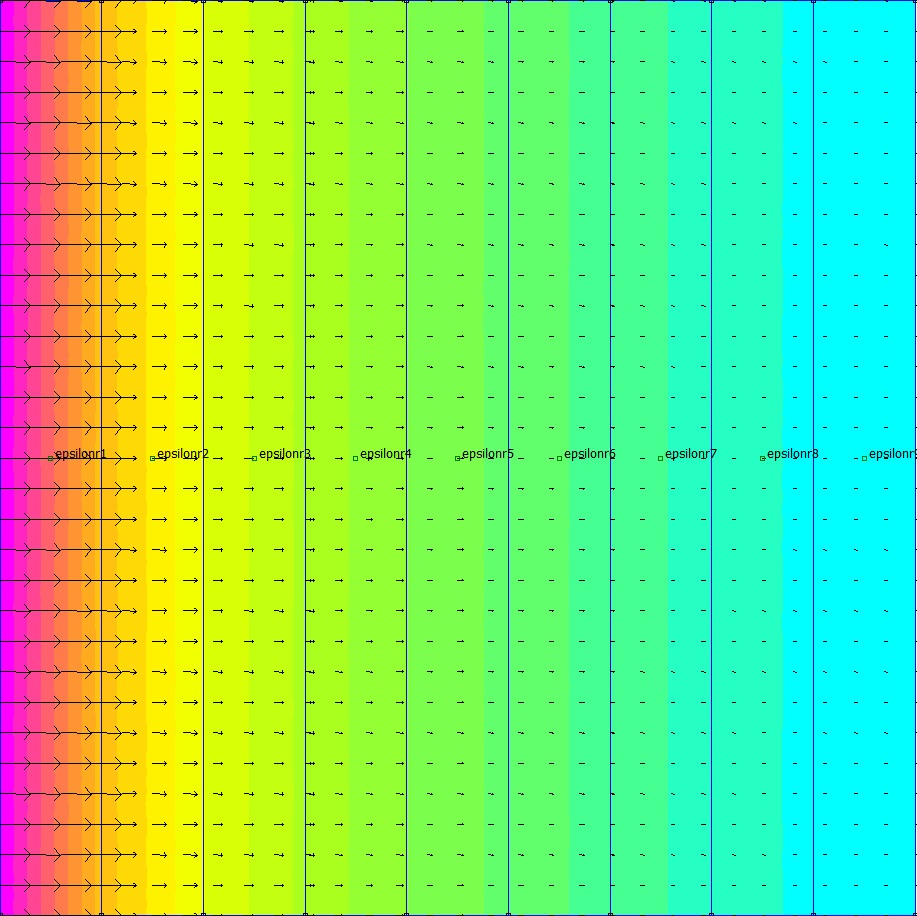
\includegraphics[width=\textwidth]{data/KondensatorN9_EFeld}
		\caption{Potentialverlauf und elektrische Feldstärke im Plattenkondensator mit 9 Schichten}
		\label{fig:N9_EFeld}
\end{subfigure}
	\caption{Potentialverlauf und elektrische Feldstärke im homogenen und im geschichteten Plattenkondensator}
\end{figure}

Bestimmt man die Kapazität für $\varepsilon_{\mathrm{r,1}} = 1$ und $\varepsilon_{\mathrm{r,2}} = 10$ und $N = 9$ und vergleicht diese mit der vorher bestimmten Kapazität $C_1$ stellt man fest, dass durch eine höhere relative Permittivität auch die Kapazität von $\SI{3,793}{\pico\farad}$ auf $\SI{8,916}{\pico\farad}$ steigt.


	%%%%%%%%%%%%%%%%%%%%%%%%%%%%%%%%%%%%%%%%%%%%
	
	%%%%%%%%%%%%%%%%%%%%%%%%%%%%%%%%%%%%%%%%%%%%%%%%%%%%%%%%%%%%%%%%%%%%%%%%%%%%%%%%%%%%%%%%%%%%%%%%%%
	
	%%%%%%%%%%%%%%%%%%%
	%Abbildungs- und Tabellenverzeichnis
	%%%%%%%%%%%%%%%%%%%
	\listoffigures % Abbildungsverzeichnis (captions in den Figuren werden als Referenz genommen)
	\listoftables % Verzeichnis der Tabellen (captions in den Tabellen werden als Referenz genommen)
	
	%%%%%%%%%%%%%%%%%%%
	%Literaturverzeichnis an dieser Stelle
	%%%%%%%%%%%%%%%%%%%
	
	
\end{document}
